\chapter{System Architecture}

This chapter presents the overall architecture and methodology of the proposed AI-powered crop disease detection system. It describes the complete research workflow, including dataset preparation, model development, ensemble learning techniques, and the experimental setup used to evaluate different deep learning architectures.

%------------------------------------------------

\section{Requirement Analysis}

The proposed AI-powered crop disease detection system was developed to automatically identify diseases affecting rice, potato, and wheat crops using deep learning techniques. Before designing and implementing the system, the functional capabilities and quality requirements were identified to ensure that the proposed solution satisfies the intended objectives. The system requirements are categorized into functional requirements and non-functional requirements.

\subsection{Functional and Non-functional Requirements}

Functional requirements describe the core functionalities that the proposed system must perform, whereas non-functional requirements define the quality attributes and operational characteristics expected from the system.

\subsubsection{Functional Requirements}

The functional requirements of the proposed system are presented in Table~\ref{tab:functional_requirements}.

\begin{table}[H]
\centering

\label{tab:functional_requirements}
\begin{tabular}{|c|p{4cm}|p{8cm}|}
\hline
\textbf{ID} & \textbf{Requirement} & \textbf{Description} \\ \hline
FR1 & Image Input & The system shall accept a leaf image of rice, potato, or wheat as input for disease identification. \\ \hline
FR2 & Image Preprocessing & The system shall resize the input image to $224 \times 224$ pixels before classification. \\ \hline
FR3 & Disease Classification & The system shall classify the input image into one of the 15 predefined disease classes. \\ \hline
FR4 & Prediction Generation & The system shall generate the predicted disease category using the trained deep learning model. \\ \hline
FR5 & Multi-Crop Support & The system shall support disease detection for rice, potato, and wheat crops. \\ \hline
FR6 & Model Evaluation & The system shall evaluate the trained models using the reserved unseen test dataset and standard evaluation metrics. \\ \hline
\end{tabular}
\caption{Functional Requirements of the Proposed System}
\end{table}

\subsubsection{Non-functional Requirements}

The non-functional requirements describe the quality attributes that the proposed system should satisfy. These requirements are summarized in Table~\ref{tab:nonfunctional_requirements}.

\begin{table}[H]
\centering

\label{tab:nonfunctional_requirements}
\begin{tabular}{|c|p{4cm}|p{8cm}|}
\hline
\textbf{ID} & \textbf{Requirement} & \textbf{Description} \\ \hline
NFR1 & Accuracy & The system should achieve high classification accuracy on unseen crop leaf images. \\ \hline
NFR2 & Reliability & The system should produce consistent predictions for similar input images. \\ \hline
NFR3 & Scalability & The architecture should allow additional crops or disease classes to be incorporated in the future. \\ \hline
NFR4 & Maintainability & The modular architecture should support easy retraining and model updates. \\ \hline
NFR5 & Usability & The trained model should be suitable for deployment in a user-friendly desktop or mobile application. \\ \hline
NFR6 & Efficiency & The system should perform disease prediction within a reasonable execution time on standard computing hardware. \\ \hline
\end{tabular}
\caption{Non-functional Requirements of the Proposed System}
\end{table}

% Keep this section concise.
% 1-2 pages maximum.

\section{Detailed Methodology and Design}

\subsection{Overall Research Workflow}

\begin{figure}[H]
    \centering
    % Change 'workflow_screenshot.png' to whatever you name the file in your img folder
    % \textwidth makes it scale perfectly to the width of your page margins
    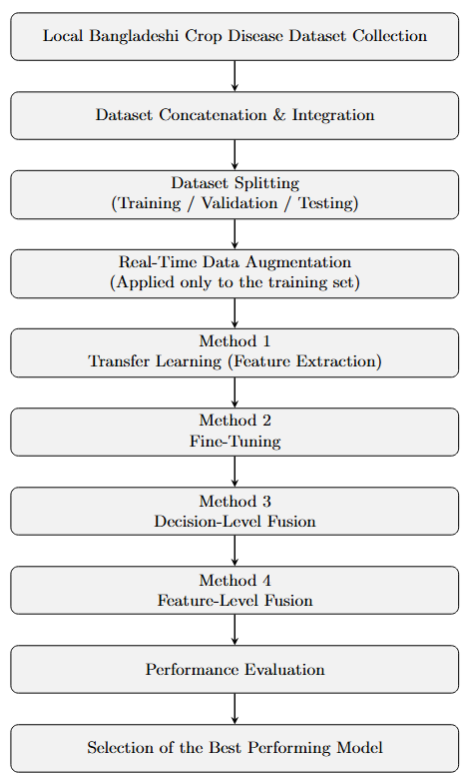
\includegraphics[width=0.6\textwidth]{img/Overall_Workflow.png} 
    \caption{Overall research workflow for the proposed crop disease detection system.}
    \label{fig:research_workflow} % Keep this label identical to your old code!
\end{figure}


\subsection{Dataset Collection}

One of the crucial factors for the effectiveness of deep learning models is the quality and variability of training data. As our focus is to design a crop disease detection model that is efficient in Bangladesh agricultural context, instead of solely relying on the commonly used PlantVillage dataset, we carefully chose publicly available crop disease datasets that are specific to our context, to ensure better generalizability in real-world scenario in Bangladeshi agriculture.

To assemble our dataset, we sourced images of crop diseases from publicly accessible platforms like Kaggle and Mendeley Data. Our assembled dataset include images of three economically important crops in Bangladesh – rice, potato and wheat – acquired from natural fields conditions.

The aforementioned datasets are selected because they feature an array of distinct disease classes, and include natural environment images and are labelled appropriately for use in deep learning based classification.

\begin{table}[H]
\centering
\begin{tabular}{|l|l|l|l|l|} 
\hline
\textbf{Dataset} & \textbf{Crop} & \textbf{Platform} & \textbf{Images} & \textbf{Environment} \\ \hline
Rice Leaf Diseases & Rice & Kaggle & $\sim$1,701 & Natural (BD) \\ \hline
Paddy Doctor & Rice & Kaggle & Subset & Mixed \\ \hline
Potato Leaf Disease & Potato & Mendeley & 3,076 & Uncontrolled \\ \hline
Wheat Disease & Wheat & Mendeley & 1,603 & Field (BD) \\ \hline
\end{tabular}
\caption{Overview of the source datasets used to compile the integrated training dataset.}
\label{tab:dataset_sources}
\end{table}


Rather than using a single dataset as it’s prevalent in the literature, in this study, multiple datasets of each crop are combined to form a single integrated dataset of varied disease conditions experienced by farmers in a practical environment. For each of the three target crops rice, potato and wheat exactly five distinct classes (including healthy and diseased states) were selected, resulting in a total of 15 classification categories. Irrelevant, highly similar, or underrepresented classes from the original sources were excluded. In summary, the integrated dataset comprises of about 6551 images classified into 15 classes and these images are ready for pre-processing, model training and evaluation steps.


\subsection{Dataset Integration}

% Explain concatenation
% Explain why PlantVillage was not used

Originally, all the collected datasets were acquired from separate public datasets with distinct directory structures, file names, and disease types. They were designed separately for different objectives so could not be used directly as a combined training data source to train a single deep learning model. The dataset integration stage combined these separate datasets into a single integrated dataset for comparative experimental comparisons. 
This created dataset contained 15 classes for 3 main crop types: potato, rice and wheat, with no specific divisions for training set, validation set, or testing set in this initial stage. 

To construct the unified dataset, a new root directory was created, and images from the selected rice, potato, and wheat datasets were reorganized according to their corresponding disease categories. Each disease category was placed into an individual class folder using a standardized naming convention, such as \texttt{potato\_early\_blight}, \texttt{rice\_blast}, and \texttt{wheat\_leaf\_blight}. This organization ensured that all crop species and disease classes followed a consistent folder hierarchy, allowing the dataset to be easily processed by TensorFlow's directory-based data loading utilities.

Images for all classes were pooled into the unified dataset. Splits were performed during the preprocessing phase later to make sure that all the experiment procedures used the same distribution of dataset.

\begin{figure}[H]
    \centering
    % Change 'workflow_screenshot.png' to whatever you name the file in your img folder
    % \textwidth makes it scale perfectly to the width of your page margins
    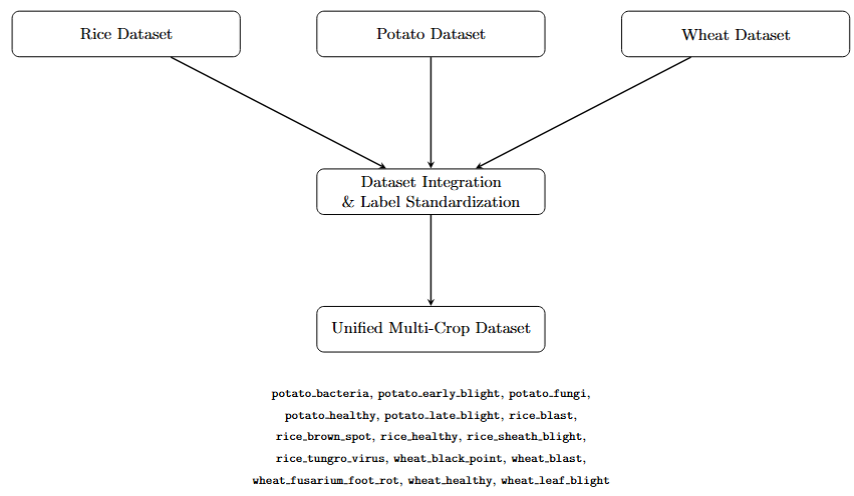
\includegraphics[width=0.85\textwidth]{img/Data_integration.png} 
   \caption{Dataset integration process from individual crop datasets into a unified multi-crop collection.}
    \label{fig:research_workflow} % Keep this label identical to your old code!
\end{figure}

The four individual datasets were merged into a single unified multi-crop repository. Classes with similar disease manifestations were standardized where possible, while preserving crop-specific distinctions. This integration created a more diverse and challenging dataset for training generalized models.

%%%FIGURE.............

\subsection{Data Preprocessing and Augmentation}

The integrated dataset then went through the complete preprocessing and augmentation process before feeding it to the model training process. This is performed so that all experimental approaches are trained and tested under exactly the same circumstances and so we are able to properly compare between the transfer learning and ensemble learning approaches tested in this study.

Following the dataset integration stage, consisting of \textbf{6,551} images across 15 disease classes, was partitioned into training, validation, and testing subsets using a \textbf{70\%-15\%-15\%} split ratio. Consequently, \textbf{4581} images were allocated to the training set, \textbf{978} images to the validation set, and \textbf{992} images to the testing set. Partitioning was done strata-wise for equal class distribution among subsets so that every disease category appeared at all experimental stage proportionaly.

Following dataset partitioning, all images underwent a unified preprocessing procedure before being supplied to the deep learning models. Since DenseNet121, MobileNetV2, and EfficientNetB0 require a fixed input resolution, every image was resized to \textbf{$224 \times 224$} pixels and processed using a batch size of 16. In contrast to traditional preprocessing pipelines where a single, global pixel normalization is applied before model inputs, the herein proposed pipeline left the pixel intensities of the data at the original levels within the data generator, letting the CNN models carry out their respective internal, model-specific preprocessing, hence perfectly fitting to the specific input needs of the different transfer learning models used.

To ensure the models generalize well to unseen images, thereby minimizing the possibility of over-fitting to the training images, real-time data augmentation was applied to the training dataset only by TensorFlow’s \texttt{ImageDataGenerator}. Instead of pre-generating and storing augmented images on disk, augmentation was applied to the images on-the-fly for every training epoch. This technique ensured a unique set of augmented images were encountered per epoch and reduced the required storage space. The training image dataset was augmented by random spatial and photometric transformations to mimic real-world agricultural field settings:

\begin{itemize}
\item Random rotations of up to $25^\circ$.
\item Horizontal and vertical translations of up to 15%.
\item Random zooming of up to 15%.
\item Shearing transformations of up to 10%.
\item Brightness variation between 80% and 120%.
\item Horizontal flipping with nearest-neighbor filling for newly created pixels.
\end{itemize}

Unlike the training dataset, both the validation and testing datasets remained completely unaugmented. This ensured that model performance was evaluated using unseen images without artificial modifications, providing an unbiased assessment of the models' generalization capability.

Finally, as the aggregated dataset had unequal numbers of images per disease category, we applied a class-weighting technique when training the model. The class weights were determined via Scikit-learn’s “balanced” approach (based on the number of samples per class), and this value was passed to the training procedure. Since under-represented classes receive a higher loss in backpropagation, the proposed methodology lessens bias to majority class, resulting in more consistent and less biased classification across all 15 classes.

% Image resizing
% Label encoding
% Train/Validation/Test split



\subsection{Transfer Learning (Feature Extraction)}

Transfer learning with feature extraction The first experimental setup for this work involved transfer learning with feature extraction. The pre-trained CNN models considered here were DenseNet121, MobileNetV2, and EfficientNetB0, used as the backbone architecture. The models were trained on ImageNet with 1000 classes and as we want to classify only 15 types of crops diseases, the original 1000-class classification layer was removed using \texttt{include\_top=False} and a new classifier was appended for the crop disease dataset of 15 classes. 

During this phase, all the weights of pre-trained backbone models were frozen. 



\begin{figure}[H]
    \centering
    % Change 'workflow_screenshot.png' to whatever you name the file in your img folder
    % \textwidth makes it scale perfectly to the width of your page margins
    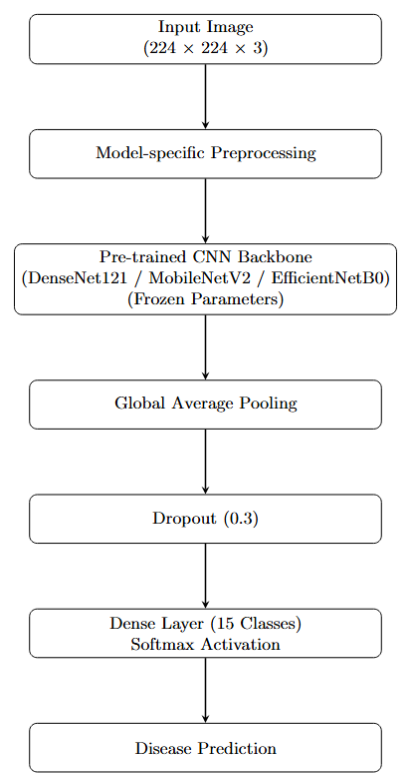
\includegraphics[width=0.65\textwidth]{img/Transfer_Learning.png} 
    \caption{Architecture of the Transfer Learning (Feature Extraction) pipeline.}
    \label{fig:research_workflow} % Keep this label identical to your old code!
\end{figure}

Only the weights of newly added classifier layers were trained. This classifier has a Global Average Pooling layer, a Dropout layer with dropout rate 0.3, and finally a Dense layer with 15 units and Softmax activation. For optimization, Adam was used with learning rate 0.001 and categorical cross-entropy as loss function. Early Stopping, Reduce Learning Rate on Plateau, and Model Checkpoint callbacks were used to monitor performance during training and to avoid overfitting. 

This experiment is performed to get the initial baseline score for each model before applying fine-tuning and ensemble.




% DenseNet
% MobileNet
% EfficientNet

\subsection{Fine-Tuning}

Post feature extraction stage A fine-tuning strategy was used to enhance the performances of the pre-trained CNN models. The previously trained DenseNet121, MobileNetV2, and EfficientNetB0 models were loaded. The convolutional backbone of each pre-trained model was partially unfrozen to be further trained on the joint crop disease data.

Only the upper layers of each backbone model were unfrozen while the previous lower layers remained frozen. It means the model adjusted its higher-level feature extraction capabilities on local crop disease images rather than completely retraining the whole network, so the general visual features gained on ImageNet are kept.
The models were recompiled with Adam optimizer and an extremely small learning rate of $1 \times 10^{-5}$. The models were then re-trained for several epochs with the same training/validation set split and class weight configuration used in the feature extraction phase. Model Checkpoint, Early Stopping, and Reduce Learning Rate on Plateau methods were once more employed to obtain the best performance.


\begin{figure}[H]
    \centering
    % Change 'workflow_screenshot.png' to whatever you name the file in your img folder
    % \textwidth makes it scale perfectly to the width of your page margins
    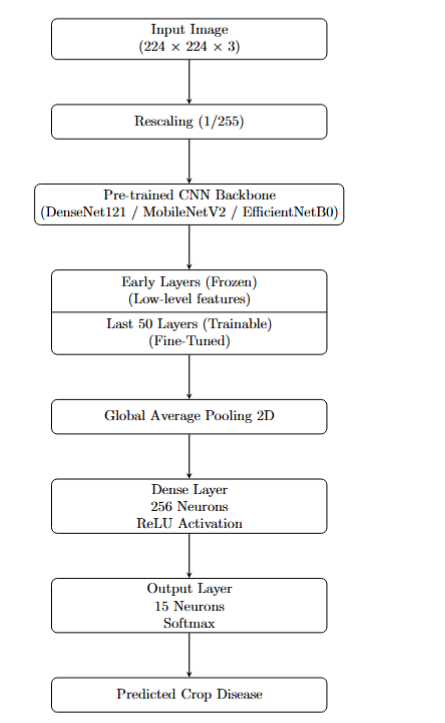
\includegraphics[width=0.65\textwidth]{img/Fine_tuning.png} 
   \caption{Architecture of the Fine-Tuning approach.}
    \label{fig:research_workflow} % Keep this label identical to your old code!
\end{figure}

This stage's purpose was to explore if partially training pre-trained backbones improves the classification performance compared to the feature extraction phase, prior to the proposal of feature-level and decision-level fusion methods.






% Explain unfreezing
% Small learning rate
\subsection{Decision-Level Fusion}

For enhance classification performance in overall. A Decision-Level Fusion method was introduced by combine all of the knowledge of the three CNNs fined-tune model(DenseNet121, MobileNetV2, EfficientNetB0) knowledge. Instead of a single model, the presented architecture utilize of prediction output of all three expert networks to make a final prediction. 

The three fine-tuned models were first loaded and their weights were frozen to preserve the knowledge acquired during the previous training stage. A unified input layer was then created, where model-specific preprocessing was applied internally. The processed inputs were simultaneously forwarded to the three expert networks, producing prediction vectors for each model.

Next, all prediction vectors from three backbone model were concatenated in to one feature presentation and feed into Dense layer with 64 neurons with relu activation, and then applied Dropout layer with 0.2 and finally Softmax layer with 15 neurons outputted the prediction disease. During training, Adam optimizer and categorical cross-entropy loss function were used with all backbone models frozen, except only the new added fusion classifier layer was optimized.

Our goal is to make full use of the different specialties of three CNNs architectures and improve the classification accuracy better than single transfer learning and fined-tuned models.

\begin{figure}[H]
    \centering
    % Change 'workflow_screenshot.png' to whatever you name the file in your img folder
    % \textwidth makes it scale perfectly to the width of your page margins
    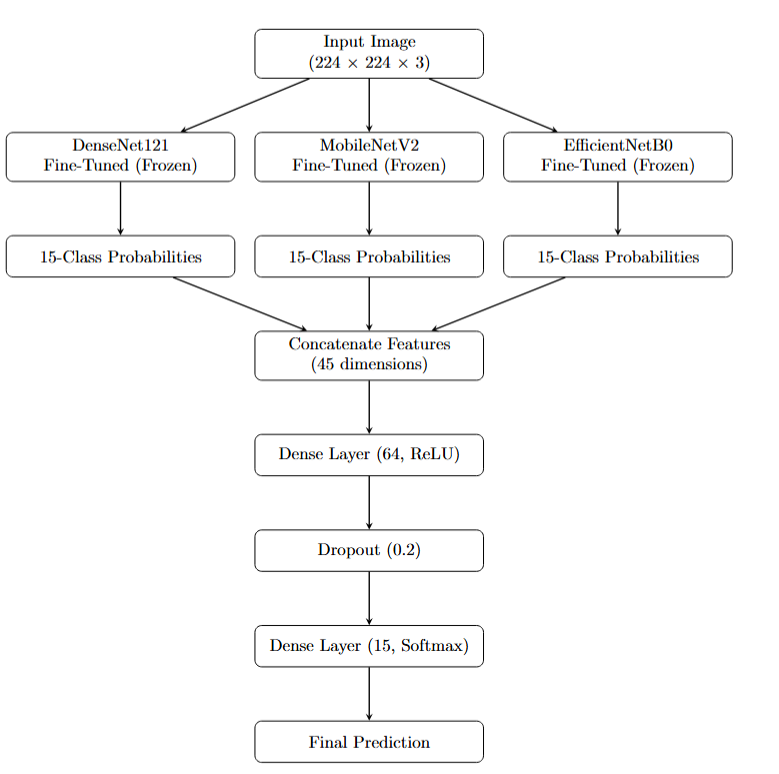
\includegraphics[width=0.75\textwidth  height=15cm, keepaspectratio]{img/Decision_level_Arc.png} 
    \label{fig:research_workflow} % Keep this label identical to your old code!
    \caption{Decision-Level Fusion architecture combining multiple CNN backbones.}
\end{figure}



% Meta learner architecture
% Diagram

\subsection{Feature-Level Fusion}

To further improve the classification performance, a feature-level fusion approach was proposed by combining the deep feature representations extracted from the three fine-tuned CNN models: DenseNet121, MobileNetV2, and EfficientNetB0. In this approach, instead of the direct prediction scores, we chose to directly feed the extracted high level feature vectors from each backbone.

Initially, three of the fine-tuned models (those with modified feature extraction layers) were utilized to extract deep feature representations for each of the images from the training and validation sets. These representations were cached on disk so that they did not have to be recalculated with each subsequent run of training, minimizing compute time and GPU RAM consumption. The features from the models were of different sizes; these were compressed into a unified 256-dimensional feature vector via fully connected layers. 

Thus, the 1024-dimensional features from DenseNet121, and the 1280-dimensional features from MobileNetV2 and EfficientNetB0, were all down-sampled to 256. 

After each such layer, batch normalization, a ReLU activation function and Dropout were used to stabilize the features and prevent over-fitting.

\begin{figure}[H]
    \centering
    % You can adjust the 8cm to whatever height looks best.
    % keepaspectratio prevents the image from looking stretched or squished!
    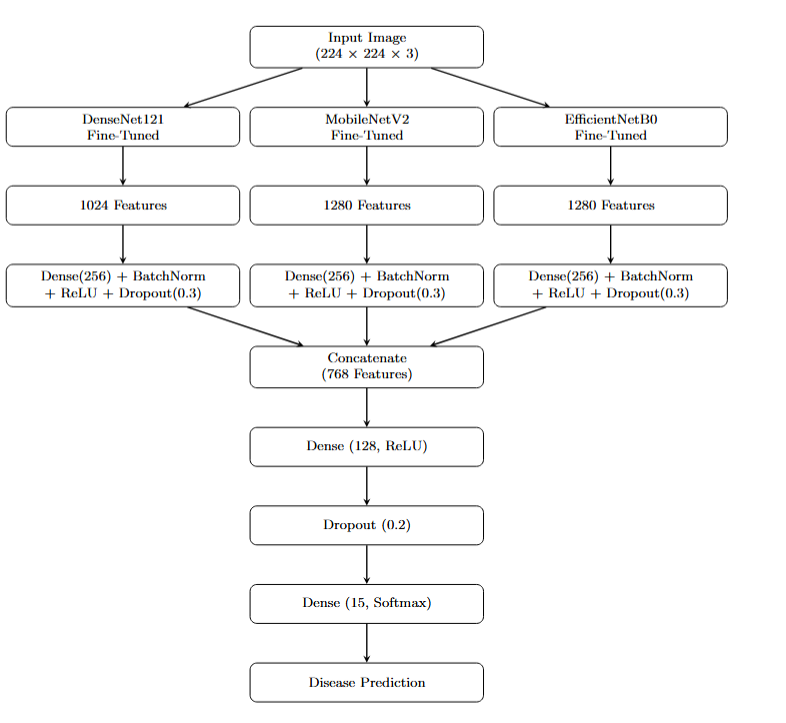
\includegraphics[width=0.85\textwidth, height=15cm, keepaspectratio]{img/Feature_level_Arc.png} 
    \caption{Feature-Level Fusion architecture with individual dense heads before concatenation.}
    \label{fig:feature_level_fusion} 
\end{figure}

Finally, the three compressed feature vectors were concatenated into a 768-dimensional feature representation that was fed into the last fusion classifier. This fusion classifier was composed of a Dense layer with 128 neurons followed by a Dropout layer and a Softmax output layer with 15 neurons, which represent the disease classes. The entire fusion classifier was trained with Adam optimizer using categorical cross-entropy loss, whereas the feature extraction networks are not updated.

The goal of this approach was to leverage the complementary feature representations captured by the three CNN architectures to obtain a more discriminative feature space for crop disease classification. 

Feature-level fusion combines deep features extracted from multiple fine-tuned CNN backbones before the final classification head. The architecture is shown below:




% 768-feature architecture
% Diagram

%------------------------------------------------


% Large workflow diagram
% 768-feature architecture
% Diagram

%------------------------------------------------

\section{Tools and Technologies Used}

The proposed crop disease detection system was developed using several software tools, programming libraries, and hardware resources. These technologies were utilized throughout the stages of dataset preprocessing, model training, evaluation, and visualization. Table~\ref{tab:tools_technologies} summarizes the major tools and technologies used in this research.

\begin{table}[H]
\centering

\label{tab:tools_technologies}
\begin{tabular}{|p{4cm}|p{10cm}|}
\hline
\textbf{Tool / Technology} & \textbf{Purpose} \\ \hline
Python 3.10 & Primary programming language used for model development and experimentation. \\ \hline
TensorFlow & Deep learning framework used for model training, fine-tuning, and inference. \\ \hline
Keras API & High-level API of TensorFlow used for constructing and training CNN models. \\ \hline
NumPy & Numerical computations and array manipulation. \\ \hline
Scikit-learn & Dataset utilities, class weight computation, and performance evaluation metrics. \\ \hline
Matplotlib & Visualization of training curves and experimental results. \\ \hline
Seaborn & Generation of confusion matrix heatmaps. \\ \hline
OpenCV & Image processing and manipulation during experimentation. \\ \hline
Visual Studio Code & Integrated Development Environment (IDE) used for implementation. \\ \hline
CUDA & GPU acceleration for deep learning model training. \\ \hline
cuDNN & GPU-optimized deep learning library used with TensorFlow. \\ \hline
\end{tabular}
\caption{Tools and Technologies Used}
\end{table}

The experiments were conducted on a personal computer equipped with an AMD Ryzen 5 5600H processor, 8 GB RAM, and an NVIDIA GeForce GTX 1650 GPU with 4 GB dedicated graphics memory. This hardware configuration provided sufficient computational capability for training and evaluating the proposed deep learning models.
% Python
% TensorFlow
% Keras
% VS Code
% HP Victus
% NVIDIA GTX 4GB
% CUDA
% OpenCV
% NumPy
% Pandas
% Matplotlib

%------------------------------------------------

\section{Work Division and Team Management}

The development of the proposed system was distributed among the three team members to ensure efficient execution across all phases of the project. Table \ref{tab:work_division} summarizes the core responsibilities assigned to each member.


\begin{table}[H]
\centering
\label{tab:work_division}
\renewcommand{\arraystretch}{1.3}
\begin{tabular}{|p{5.5cm}|c|c|c|}
\hline
\textbf{Task} & \textbf{Md. Shihab PK} & \textbf{Md. Shohan Uzzaman} & \textbf{Md. Sohel Rana} \\
\hline
Literature Review & \checkmark & \checkmark & \checkmark \\
\hline
Dataset Collection and Integration & & \checkmark & \checkmark \\
\hline
Data Preprocessing and Augmentation & & \checkmark & \checkmark \\
\hline
Transfer Learning Model Development & \checkmark & & \\
\hline
Fine-Tuning of CNN Models & \checkmark & & \\
\hline
Decision-Level Fusion Development & \checkmark & & \\
\hline
Feature-Level Fusion Development & \checkmark & & \\
\hline
Model Evaluation and Performance Analysis & \checkmark & \checkmark & \\
\hline
User Interface and Application Integration & & & \checkmark \\
\hline
Result Analysis and Discussion & \checkmark & \checkmark & \checkmark \\
\hline
Thesis Writing and Documentation & \checkmark & \checkmark & \checkmark \\
\hline
Final Review and Presentation Preparation & \checkmark & \checkmark & \checkmark \\
\hline
\end{tabular}
\caption{Work Division Among Team Members}
\end{table}
% Table

%------------------------------------------------

\section{Time Frame}

To ensure a structured and timely progression of the thesis, the project was divided into distinct developmental phases. Table \ref{tab:time_frame} illustrates the schedule, highlighting the major milestones achieved over the course of the final academic year.

\begin{table}[H]
\centering
\label{tab:time_frame}
\renewcommand{\arraystretch}{1.4}
\begin{tabular}{@{} l l @{}}
\toprule
\textbf{Project Phase \& Major Tasks} & \textbf{Completion Window} \\
\midrule
\textbf{Phase 1: Research \& Preparation} & \\
\hspace{0.5cm} Literature Review \& Requirement Analysis & September 2025 -- October 2025 \\
\hspace{0.5cm} Dataset Collection \& Image Preprocessing & November 2025 -- December 2025 \\
\midrule
\textbf{Phase 2: Core Development} & \\
\hspace{0.5cm} Base Model Training \& Fine-Tuning & January 2026 -- February 2026 \\
\hspace{0.5cm} Decision-Level \& Feature-Level Fusion & March 2026 -- April 2026 \\
\midrule
\textbf{Phase 3: Integration \& Finalization} & \\
\hspace{0.5cm} Application Integration \& System Testing & April 2026 -- May 2026 \\
\hspace{0.5cm} Model Evaluation \& Thesis Documentation & May 2026 -- June 2026 \\
\bottomrule
\end{tabular}
\caption{Project Time Frame and Major Milestones}
\end{table}
% Gantt Chart

%------------------------------------------------

\section{Summary}

In this chapter, we provided the detailed process and architectural design employed to produce the AI-based crop disease identification system. The research methodology commenced with detailed requirements gathering and a thorough analysis conducted to cater for functional and non-functional attributes to make the system useful in the real world. An inclusive and targeted image data of 6,551, capturing 15 types of plant diseases(including healthy) and three crops namely wheat, potato, and rice, was gathered and properly organized. After gathering, it was fused and meticulously pre-processed with the use of real-time image enhancement, on-the-fly image augmentation, and balancing classes.

The chapter then outlined the progressive deep learning strategies employed, transitioning from baseline feature extraction using DenseNet121, MobileNetV2, and EfficientNetB0, to targeted fine-tuning. Building upon these base models, two advanced ensemble architectures were detailed: a weighted decision-level fusion utilizing prediction vectors, and a highly discriminative feature-level fusion synthesizing deep morphological features. Finally, the hardware, software tools, team work division, and chronological milestones were documented to provide a transparent overview of the project's execution. With the methodological framework established.